% !Mode:: "TeX:UTF-8"
%% 请使用 XeLaTeX 编译本文.
% \documentclass{WHUBachelor}% 选项 forprint: 交付打印时添加, 避免彩色链接字迹打印偏淡. 即使用下一行:
 \documentclass[forprint]{WHUBachelor}

\begin{document}
%%%%%%% 下面的内容, 据实填空.

\miji{ }                                      % 密级. 没有就空着.
\StudentNumber{220205764} % 填写自己的学号

\title{数值分析上机报告 \\ 第二章}
\author{周玉乾}                            % 作者名字
\Cschoolname{微电子学院}          % 学院名
\date{二〇二〇年十一月}                    % 日期, 要注意和英文日期一致!!
\Edate{Nov, 2020}                       % 英文封面日期

%-----------------------------------------------------------------------------
\pdfbookmark[0]{封面}{title}         % 封面页加到 pdf 书签
\maketitle
\frontmatter
\pagenumbering{Roman}              % 正文之前的页码用大写罗马字母编号.
%-----------------------------------------------------------------------------
%% !Mode:: "TeX:UTF-8"

%%% 此部分需要自行填写: (1) 中文摘要及关键词 (2) 英文摘要及关键词
%%%%%%%%%%%%%%%%%%%%%%%%%%%%%
%%% -------------  英文封面 (无需改动)-------------   %%%
%%%%%%%%%%%%%%%%%%%%%%%%%%%%%
\thispagestyle{empty}
\renewcommand{\baselinestretch}{1.5}  %下文的行距
\vspace*{0.5cm}
\begin{center}
{\Large \bf BACHELOR'S DEGREE THESIS \\[1ex] OF WUHAN UNIVERSITY }
\end{center}
\vspace{2.5cm}
\begin{center}{\zihao{2} \the\Etitle \par}\end{center}

\vfill

\begin{center}
\zihao{4}
\begin{tabular}{ r l }
 School (Department): & {\sc \the\Eschoolname}\\
  Major:          &   {\sc\the\Emajor}  \\
 Candidate:      &  {\sc \the\Eauthor}      \\
 Supervisor:     &  {\sc \the\Esupervisor}
\end{tabular}

\vspace*{2cm}
\begin{center}
   \ifprint % 文档打印, 使用黑白校徽.
  \includegraphics[height=4cm]{whu.eps}       %%  黑白的.
  \else
  \includegraphics[height=4cm]{whulogo.eps} %%  彩色的.
  \fi
\end{center}


\zihao{-2}
%\the\Schoolname\\
{\sc Wuhan University}

\vspace*{1.0cm}

\the\Edate

\end{center}
%%% 郑重声明部分无需改动

%%%---- 郑重声明 (无需改动)------------------------------------%
\newpage
\vspace*{20pt}
\begin{center}{\ziju{0.8}\textbf{\songti\zihao{2} 郑重声明}}\end{center}
\par\vspace*{30pt}
\renewcommand{\baselinestretch}{2}

{\zihao{4}%

本人呈交的学位论文, 是在导师的指导下, 独立进行研究工作所取得的成果,
所有数据、图片资料真实可靠. 尽我所知, 除文中已经注明引用的内容外,
本学位论文的研究成果不包含他人享有著作权的内容.
对本论文所涉及的研究工作做出贡献的其他个人和集体,
均已在文中以明确的方式标明. 本学位论文的知识产权归属于培养单位.\\[2cm]

\hspace*{1cm}本人签名: $\underline{\hspace{3.5cm}}$
\hspace{2cm}日期: $\underline{\hspace{3.5cm}}$\hfill\par}
%------------------------------------------------------------------------------
\baselineskip=23pt  % 正文行距为 23 磅
%------------------------------------------------------------------------------





%%======中文摘要===========================%
\begin{cnabstract}
本文主要介绍和讨论了武汉大学本科毕业论文的~\LaTeX~模板.
指明了编译方法, 强调了公式排版的一些细节问题, 也指出了一些常见的排版错误.



\end{cnabstract}
\par
\vspace*{2em}


%%%%--  关键词 -----------------------------------------%%%%%%%%
%%%%-- 注意: 每个关键词之间用“;”分开,最后一个关键词不打标点符号
\cnkeywords{毕业论文; \LaTeX{}; 模板;  }


%%====英文摘要==========================%


\begin{enabstract}
This thesis is a study on the theory of \dots.

\end{enabstract}
\par
\vspace*{2em}

%%%%%-- Key words --------------------------------------%%%%%%%
%%%%-- 注意: 每个关键词之间用“;”分开,最后一个关键词不打标点符号
 \enkeywords{\LaTeX{};  }
    % 加入摘要, 申明.
%==========================把目录加入到书签==============================%%%%%%
%\pdfbookmark[0]{目录}{toc}
%\tableofcontents
\mainmatter %% 以下是正文
%%%%%%%%%%%%%%%%%%%%%%%%%%%--------main matter-------%%%%%%%%%%%%%%%%%%%%%%%%%%%%%%%%%%%%
%\chapter[第一章]{} % (fold)
\label{cha:chapter1}

\section{问题 \\ 舍入误差与有效数字}

设 $S_N = \sum ^N _{j=2} \frac{1}{j^2-1}$,其精确值为 $\frac{1}{2}(\frac{3}{2}-\frac{1}{N}-\frac{1}{N+1})$。

\begin{enumerate}
    \item 编制按从大到小的顺序 $S_N = \frac{1}{2^2-1} + \frac{1}{3^2-1} + ... + \frac{1}{N^2-1}$,计算 $S_N$ 的通用程序;

    \item 编制按从小到大的顺序 $S_N = \frac{1}{N^2-1} + \frac{1}{(N-1)^2-1} + ... + \frac{1}{2^2-1}$,计算 $S_N$ 的通用程序;

    \item 按两种顺序分别计算 $S_{10^2}$、$S_{10^4}$、$S_{10^6}$,并指出其有效位数(编程时用单精度);

    \item 通过本上机题你明白了什么?

\end{enumerate}

\section{分析}

对于 $\frac{1}{N^2-1}$,当 $N$ 很大时,$\frac{1}{N^2-1}$ 接近0,因此如果按从大到小的顺序计算 $S_N = \frac{1}{2^2-1} + \frac{1}{3^2-1} + ... + \frac{1}{N^2-1}$,由于计算机的舍入误差,会出现\textbf{大数吃小数}的情况,从而比真实结果略小;而如果按从小到大的顺序计算 $S_N = \frac{1}{N^2-1} + \frac{1}{(N-1)^2-1} + ... + \frac{1}{2^2-1}$,其结果应该更加接近真实值。

\section{程序}

q1-1.cpp

\begin{lstlisting}[style = cpp]
#include <iostream>
#include <iomanip>
#include <math.h>

float f(int N) {
    float res = 0;
    res = float(1.0)/(pow(float(N), float(2)) - 1);
    return res;
}

float SN_1(int N) {
    float sum = 0;
    for (int i = 2; i <= N; i++)
    {
        sum += f(i);
    }
    return sum;
}

float SN_2(int N) {
    float sum = 0;
    for (int i = N; i >= 2; i--)
    {
        sum += f(i);
    }
    return sum;
}

float SN_Real(int N) {
    float sum = 0;
    sum = 0.5*(1.5 - 1/N - 1/(N+1));
    return sum;
}

int main() {
    float data0 = 0;
    float data1 = 0;
    float data2 = 0;

    int N = 0;

    std::cout<<"请输入N:"<<std::endl;
    std::cin>>N;

    data0 = SN_Real(N);
    data1 = SN_1(N);
    data2 = SN_2(N);

    std::cout<<"N\t精确值\t\t从大到小\t误差1   \t从小到大\t误差2"<<std::endl;
    std::cout<<N<<"\t"<< std::fixed << std::setprecision(8)<<data0<<"\t"<<data1<<"\t"<<abs(data0-data1)<<"\t"<<data2<<"\t"<<abs(data0-data2)<<std::endl;

    return 0;
}
\end{lstlisting}

\section{算例}

\begin{enumerate}
    \item $S_{10^2}$

    \begin{lstlisting}[style = cpp]
$ ./q1-1
请输入N:
100
N   精确值       从大到小      误差1       从小到大      误差2
100 0.75000000  0.74004948  0.00995052  0.74004954  0.00995046
    \end{lstlisting}

    \item $S_{10^4}$

    \begin{lstlisting}[style = cpp]
$ ./q1-1
请输入N:
10000
N       精确值       从大到小      误差1       从小到大      误差2
10000  0.75000000   0.74985212  0.00014788  0.74989998  0.00010002
    \end{lstlisting}

    \item $S_{10^6}$

    \begin{lstlisting}[style = cpp]
$ ./q1-1
请输入N:
1000000
N       精确值       从大到小      误差1       从小到大      误差2
1000000 0.75000000  0.74985212  0.00014788  0.74999905  0.00000095
    \end{lstlisting}

\end{enumerate}

\section{结论}

\begin{table}[ht]
  \centering
  \caption{有效位数}
  \label{tab:1}
  \begin{tabular}{*{20}c}
     \hline
    %  \cline{col1-col2}
     N & $10^2$ & $10^4$ & $10^6$ \\
     \hline
     % after \\: \hline or \cline{col1-col2} \cline{col3-col4} ...
     从大到小 & 1  & 3  & 3 \\
     从小到大 & 1  & 3  & 5 \\
     \hline
   \end{tabular}
\end{table}

\begin{enumerate}
    \item 编程证明了之前的分析,及从大到小求和时,会出现大数吃小数的现象,导致误差偏大;

    \item 再次证明了数学上的等价并不意味着数值上的等价,在实际的运算中,舍入误差的影响不可低估,在计算中选择一种好的算法可以使结果更加精确。
\end{enumerate}



% chapter chapter1 (end)
\setcounter{chapter}{1}
\chapter[第二章]{} % (fold)
\label{cha:chapter2}

\section{问题 \\ 试值法或者Newton法同二分法结合}

\subsection{问题1} % (fold)
\label{sub:问题1}

\begin{figure}[ht]
\centering
  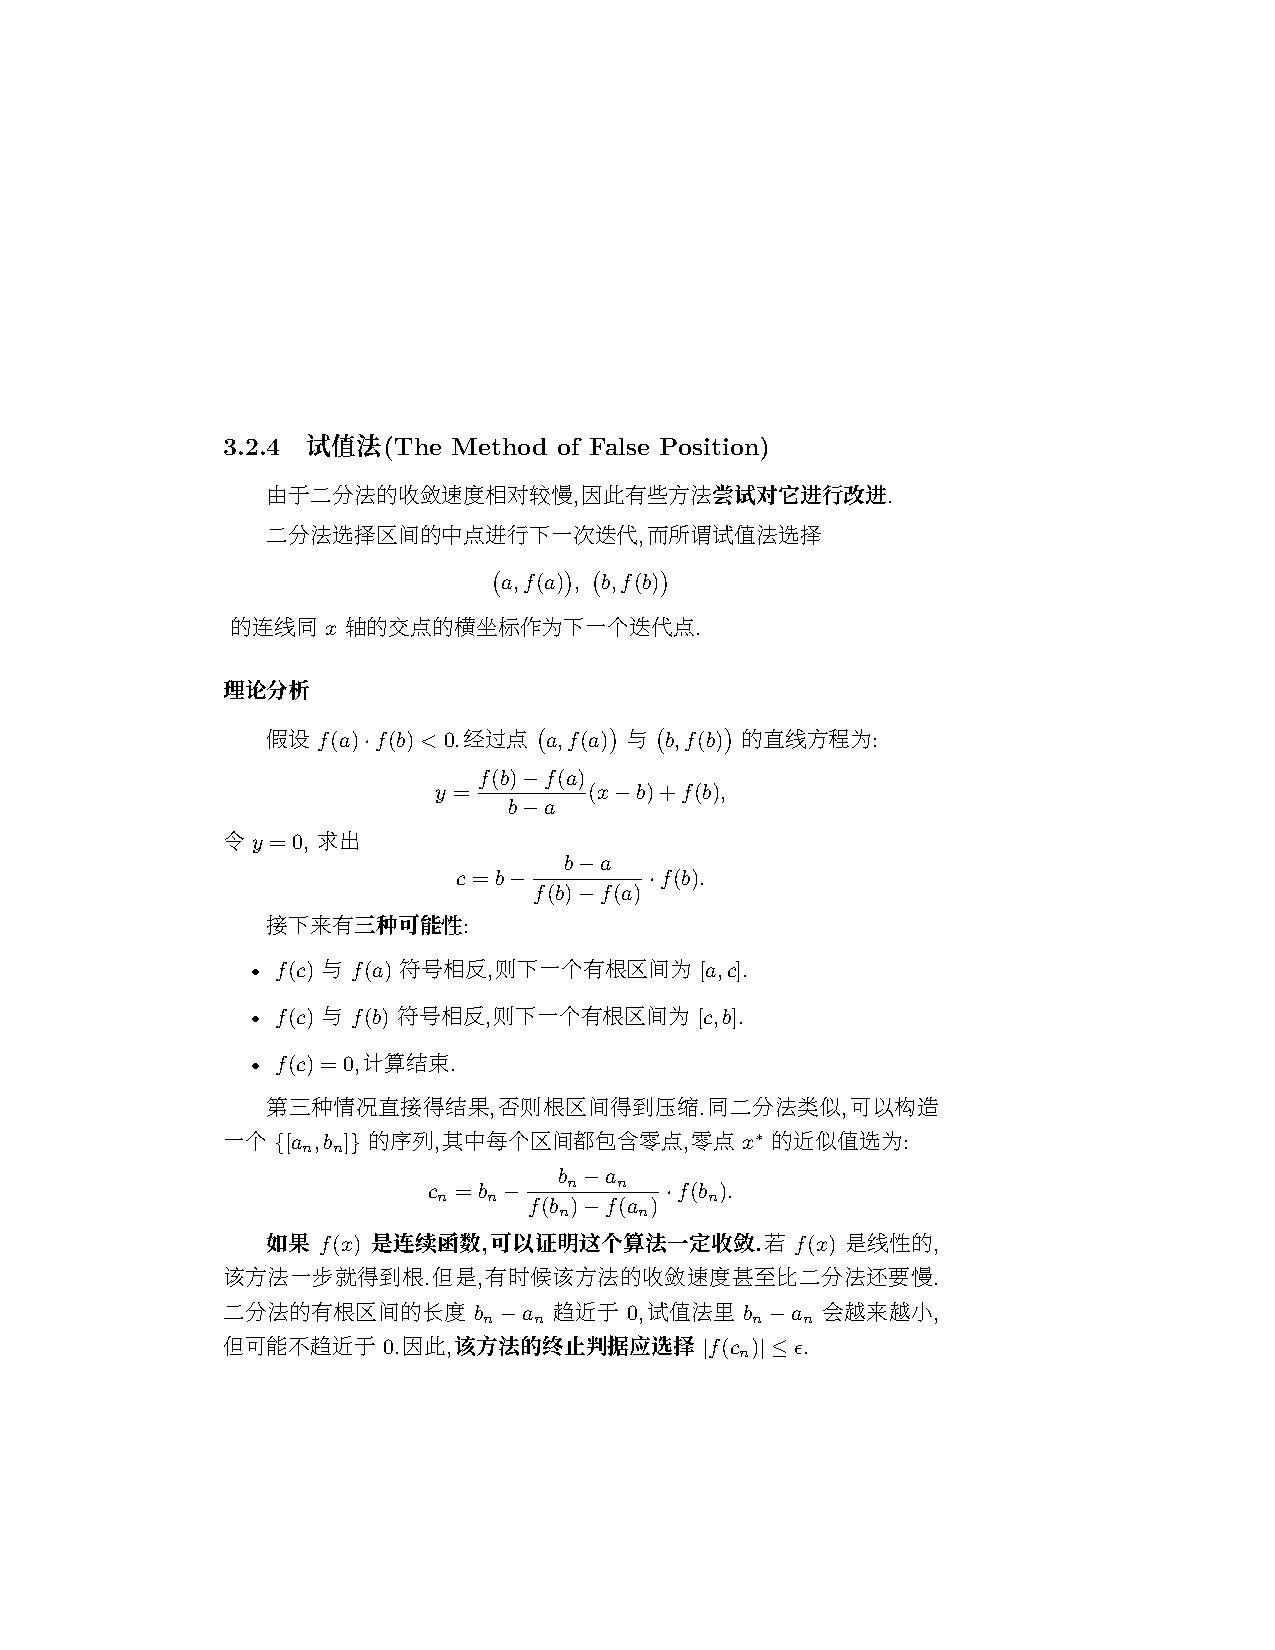
\includegraphics[width=\textwidth]{TVM}
  % \caption{试值法算法}
  % \label{fig:TVM}
\end{figure}

% subsection 问题1 (end)

\subsection{问题2} % (fold)
\label{sub:问题2}

\begin{figure}[ht]
\centering
  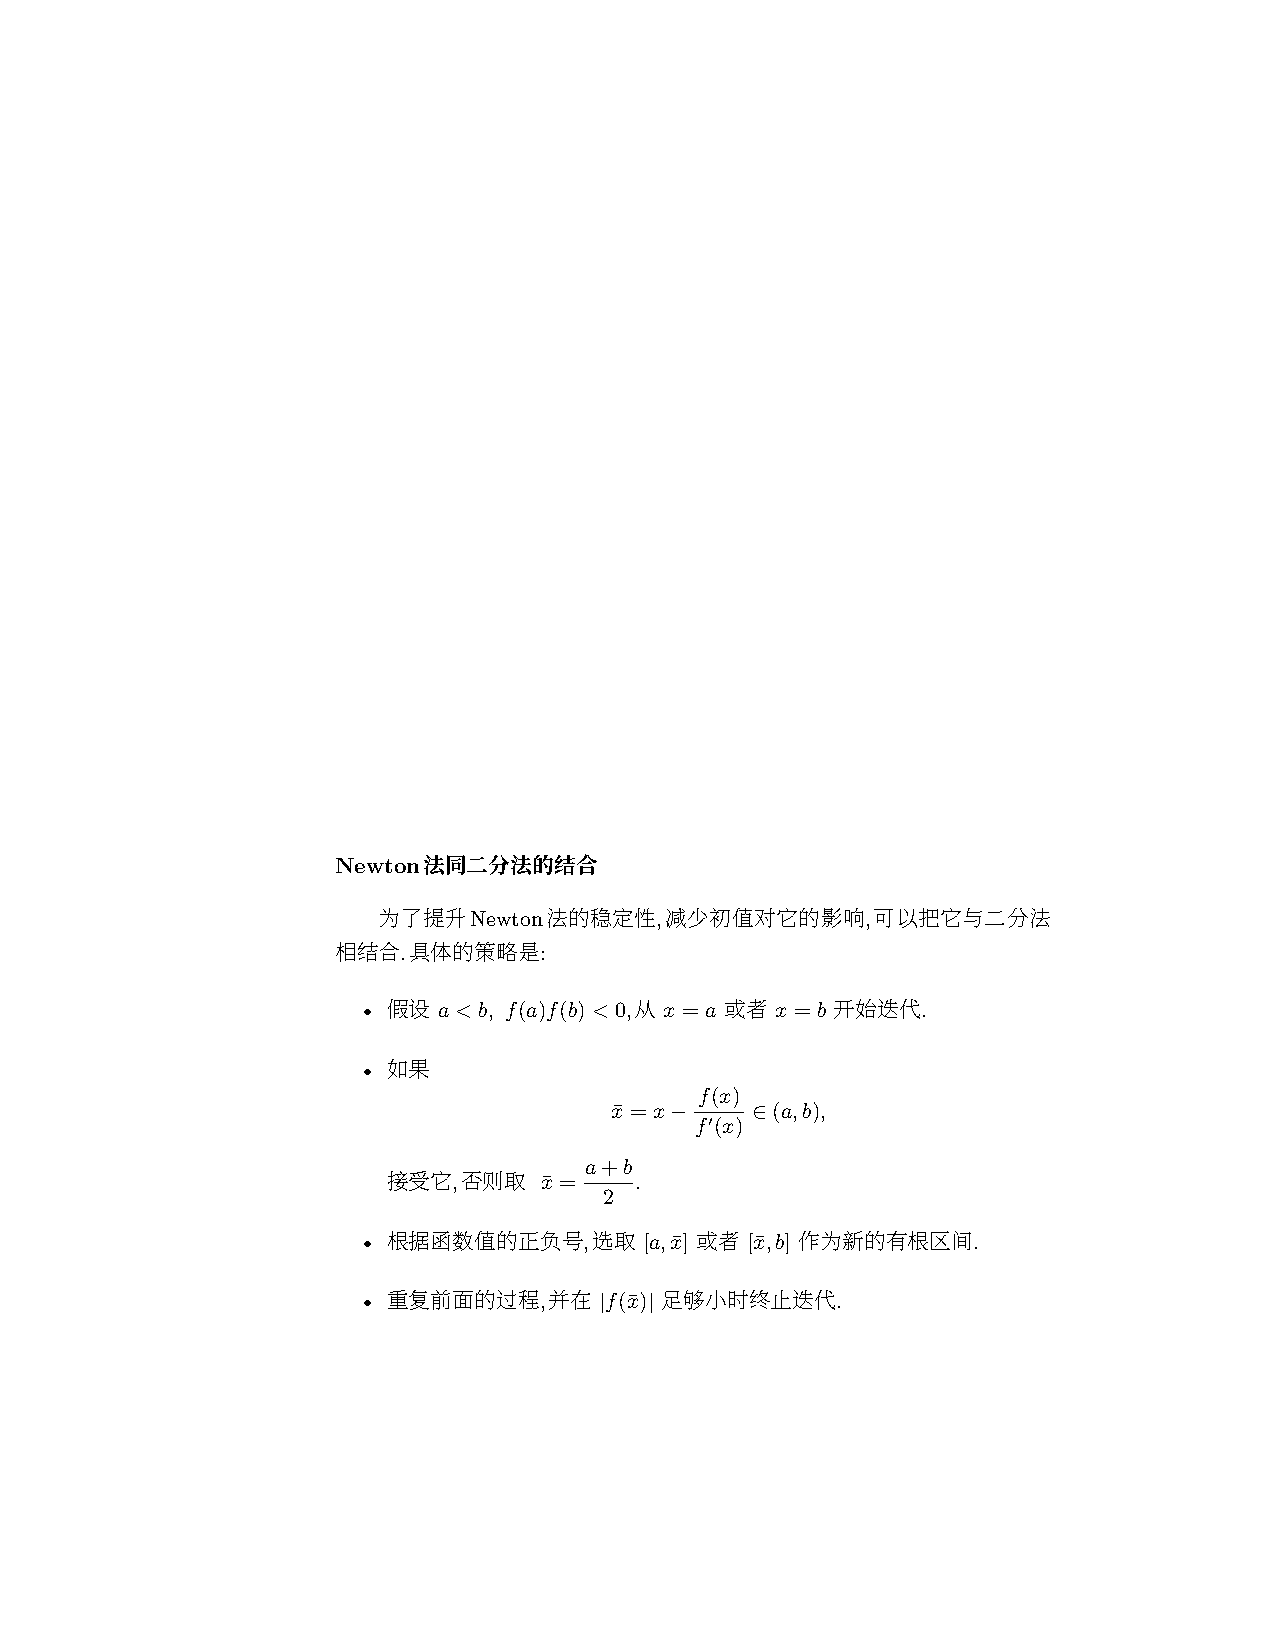
\includegraphics[width=\textwidth]{Newton}
  % \caption{Newton法同二分法结合}
  % \label{fig:Newton}
\end{figure}

% subsection 问题2 (end)


\section{分析}

\subsection{试值法流程}

图\ref{fig:TrailValueFlow} 为试值法算法流程图。

\begin{figure}[ht]
\centering
  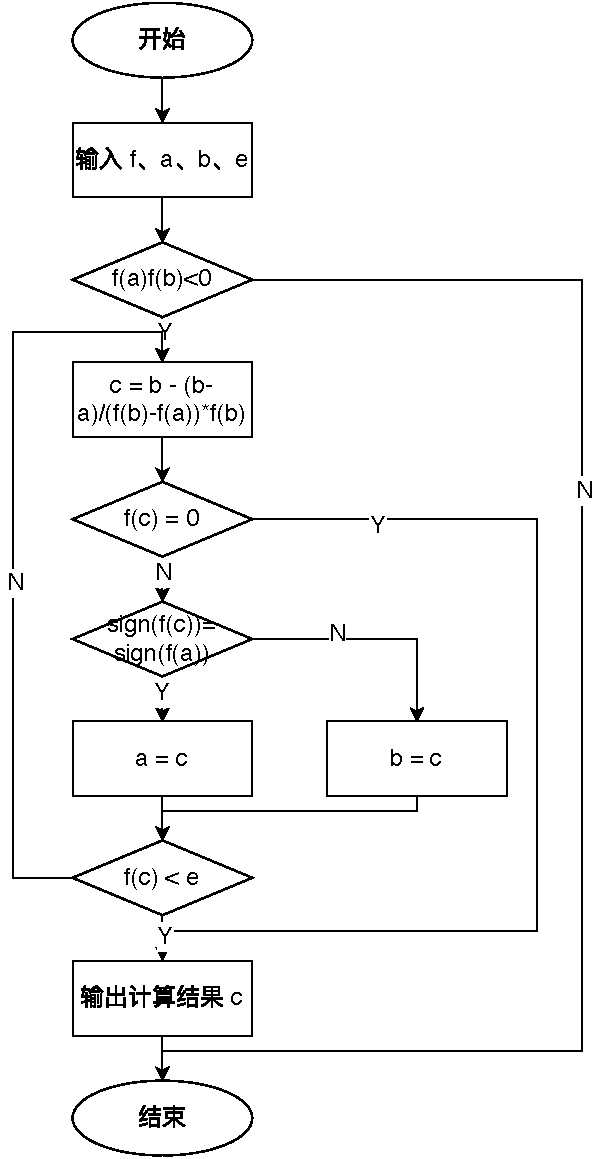
\includegraphics[width=0.5\textwidth]{TrailValueFlow}
  \caption{试值法流程图}
  \label{fig:TrailValueFlow}
\end{figure}

\subsection{Newton法同二分法结合流程}

图\ref{fig:NewtonFlow} 为试值法算法流程图。

\begin{figure}[ht]
\centering
  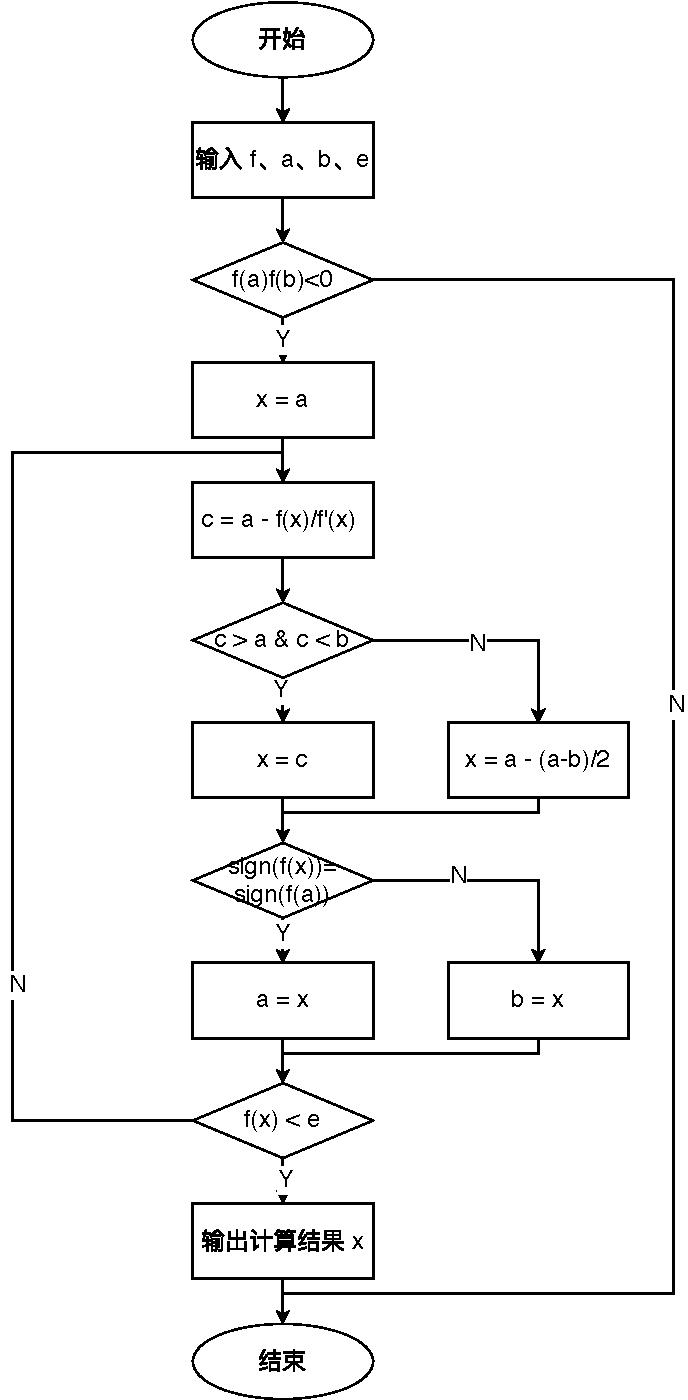
\includegraphics[width=0.5\textwidth]{Newton2Flow}
  \caption{Newton法同二分法结合流程}
  \label{fig:NewtonFlow}
\end{figure}

\section{程序}

试值法

\begin{lstlisting}[style = python]
def TrailValue(expr, a, b, e):
    """
    试值法
    f@函数
    a@区间下限
    b@区间上限
    e@容忍误差限
    """
    f = _func(expr)
    fa_0 = f.value(a)
    fb_0 = f.value(b)
    res = 0
    count = 0
    if abs(fa_0) < e:
        res = a
    elif abs(fb_0) < e:
        res = b
    elif sympy.sign(fa_0) == sympy.sign(fb_0):
        print('f(a) and f(b) 同号')
        sys.exit()
    else:
        while True:
            count = count + 1
            fa = f.value(a)
            fb = f.value(b)
            c = b - ((b-a)/(fb - fa))*fb
            fc = f.value(c)

            # 更新有根区间
            if sympy.sign(fa) == sympy.sign(fc):
                a = c
            else:
                b = c

            # 判断计算结束
            if abs(f.value(c)) < e:
                res = c
                break

    return res, count
\end{lstlisting}

Newton法同二分法结合

\begin{lstlisting}[style = python]
def Newton(expr, a, b, e):
    """
    牛顿法与二分法结合
    f@函数
    a@区间下限
    b@区间上限
    e@容忍误差限
    """
    f = _func(expr)
    fa_0 = f.value(a)
    fb_0 = f.value(b)
    res = 0
    count = 0
    if abs(fa_0) < e:
        res = a
    elif abs(fb_0) < e:
        res = b
    elif sympy.sign(fa_0) == sympy.sign(fb_0):
        print('f(a) and f(b) 同号')
        sys.exit()
    else:
        x = a
        while True:
            count = count + 1
            c = x - f.value(x)/f.diff_value(x)

            # Newton与二分法结合,找下一个点
            if (c > a) and (c < b):
                x = c
            else:
                x = a+(b-a)/2

            # 更新有根区间
            if sympy.sign(f.value(a)) == sympy.sign(f.value(x)):
                a = x
            else:
                b = x

            # 判断计算结束
            if abs(f.value(x)) < e:
                res = x
                break

    return res, count
\end{lstlisting}

\section{算例}

\begin{enumerate}
  \item $x\times sin(x) - 1 = 0$,有根区间为(1, 2),误差限为$1\times 10^{-5}$。

  \begin{lstlisting}[style = python]
  试值法 根: 1.11416, 迭代次数: 3
  牛顿法 根: 1.11416, 迭代次数: 2
  \end{lstlisting}
  
  \item $x^2 - 5 = 0$,有根区间为(2, 3),误差限为$1\times 10^{-5}$。

  \begin{lstlisting}[style = python]
  试值法 根: 2.23607, 迭代次数: 7
  牛顿法 根: 2.23607, 迭代次数: 3
  \end{lstlisting}

  \item $x^3 -3x + 2 = 0$,有根区间为(-2.5, -1.5),误差限为$1\times 10^{-5}$。

  \begin{lstlisting}[style = python]
  试值法 根: -2.00000, 迭代次数: 11
  牛顿法 根: -2.00000, 迭代次数: 4
  \end{lstlisting}

\end{enumerate}

\section{结论}

\begin{enumerate}
  \item 相比于试值法,Newton与二分法结合的算法收敛速度更快;

  \item Newton与二分法结合提升了原始Newton法的稳定性;

  \item 无论是试值法还是Newton与二分法结合的算法,都只能求解函数穿过x轴的根,不能求解函数与x轴相切的根,例如在算例3中,无法求解 $x = 1.0$ 的根。

  \begin{figure}[ht]
  \centering
    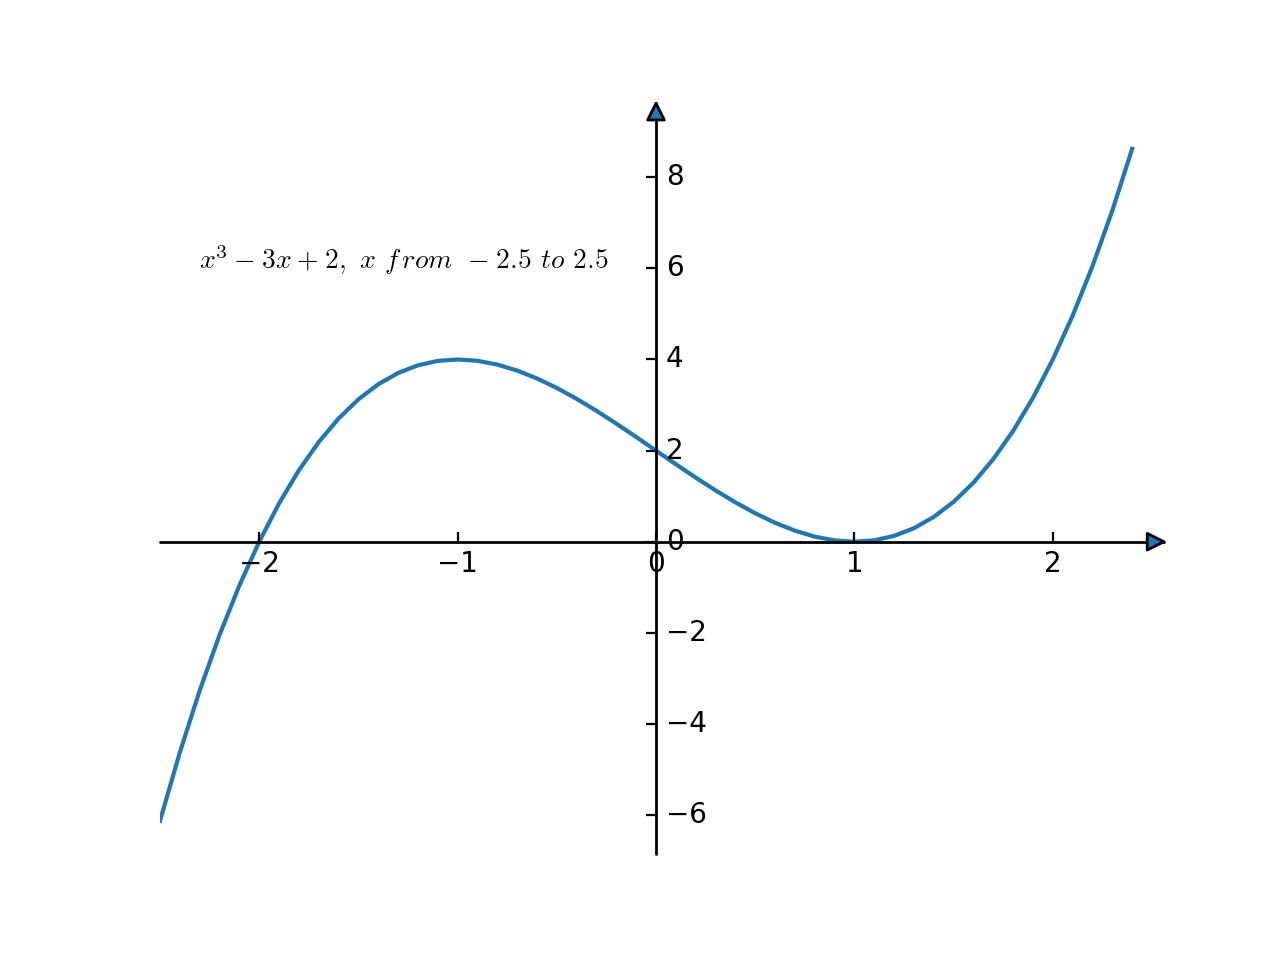
\includegraphics[width=0.6\textwidth]{f3}
    \caption{$f(x) = x^3 -3x + 2$}
    \label{fig:f3}
  \end{figure}

\end{enumerate}

% chapter chapter2 (end)
%\chapter[第三章]{} % (fold)
\label{cha:chapter3}

\section{问题 \\ 列主元 Gauss 消去}

对于某电路的分析,归结于求解线性方程组 $RI = V$,其中

$$
R = 
\begin{bmatrix}
31 & -13 & 0 & 0 & 0 & -10 & 0 & 0 & 0 \\
-13 & 35 & -9 & 0 & -11 & 0 & 0 & 0 & 0 \\
0 & -9 & 31 & -10 & 0 & 0 & 0 & 0 & 0 \\
0 & 0 & -10 & 79 & -30 & 0 & 0 & 0 & -9 \\
0 & 0 & 0 & -30 & 57 & -7 & 0 & -5 & 0 \\
0 & 0 & 0 & 0 & -7 & 47 & -30 & 0 & 0 \\
0 & 0 & 0 & 0 & 0 & -30 & 41 & 0 & 0 \\
0 & 0 & 0 & 0 & -5 & 0 & 0 & 27 & -2 \\
0 & 0 & 0 & -9 & 0 & 0 & 0 & -2 & 29
\end{bmatrix}
$$

$$
V^T = (-15, 27, -23, 0, -20, 12, -7, 7, 10)^T
$$

\begin{enumerate}
    \item 编制解 n 阶线性方程组 $Ax = b$ 的列主元 Gauss 消去的通用程序;

    \item 用所编程序解线性方程组 $RI = V$,并打印出解向量,保留5位有效数字;

    \item 本题编程之中,你提高了哪些能力?

\end{enumerate}

\section{分析}

列主元 Gauss 消去的算法流程图如图 \ref{fig:GaussFlow} 所示。

  \begin{figure}[H]
  \centering
    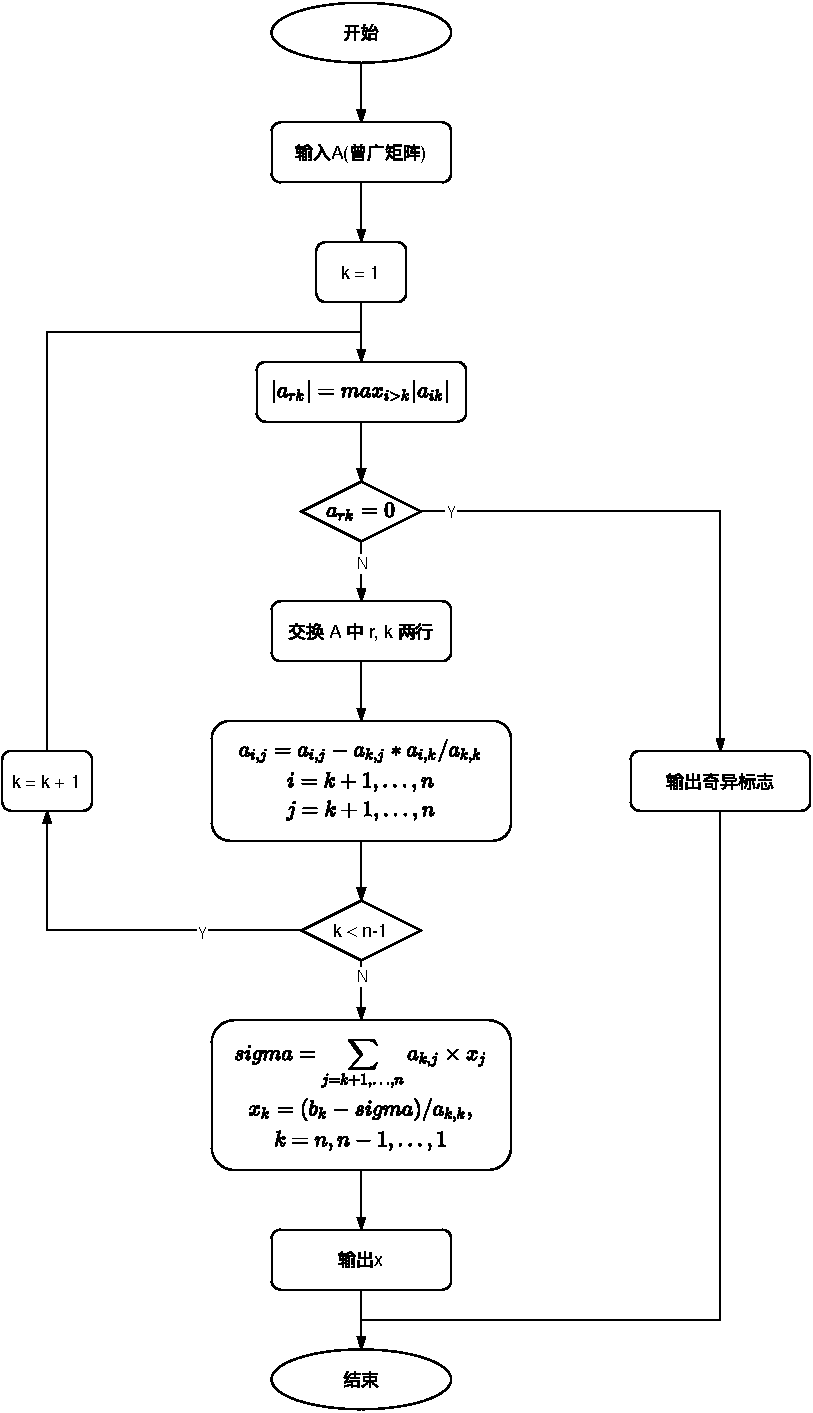
\includegraphics[width=0.7\textwidth]{GaussFlow}
    \caption{列主元 Gauss 消去算法流程}
    \label{fig:GaussFlow}
  \end{figure}

\section{程序}

\begin{lstlisting}[style = python]
import sys
import numpy as np

A = [[31, -13, 0, 0, 0, -10, 0, 0, 0],
    [-13, 35, -9, 0, -11, 0, 0, 0, 0],
    [0, -9, 31, -10, 0, 0, 0, 0, 0],
    [0, 0, -10, 79, -30, 0, 0, 0, -9],
    [0, 0, 0, -30, 57, -7, 0, -5, 0],
    [0, 0, 0, 0, -7, 47, -30, 0, 0],
    [0, 0, 0, 0, 0, -30, 41, 0, 0],
    [0, 0, 0, 0, -5, 0, 0, 27, -2],
    [0, 0, 0, -9, 0, 0, 0, -2, 29]]

b = [-15, 27, -23, 0, -20, 12, -7, 7, 10]

def find_shape(A, b):
    """
    获取 n
    """

    # n行 m列
    n1, m1 = A.shape
    n2, = b.shape

    # print(n1, m1)
    # print(n2)

    # 判断矩阵形状
    if n1 != m1 or n1 != n2:
        print('Error martix shape!')
        sys.exit()
    else:
        N = n1

    return N
    

def MGauss(A, b):
    """
    列主元 Gauss 消去 消元
    """

    # 判断矩阵形状
    N = find_shape(A, b)

    # 列主元高斯消元
    for k in range(0, N):
        p = k
        maxabs = abs(A[k, k])
        # 找列最大值
        for i in range(k+1, N):
            if abs(A[i, k]) > maxabs:
                p = i
                maxabs = abs(A[i, k])
        print('maxabs', maxabs)
        # 最大值为 0
        if maxabs == 0:
            print('Singular')
            sys.exit()
        # 最大值不在对角线, 则交换两行
        if p != k:
            A[[p,k],:] = A[[k,p],:]
            b[[p,k]] = b[[k,p]]
        print('exchange r{0} and r{1}:\r\n'.format(k, p), A)
        # 消元,将对角线以下变为 0
        for i in range(k+1, N):
            m_ik = A[i, k] / A[k, k]
            for j in range(0, N):
                A[i, j] -= A[k, j] * m_ik
            b[i] -= b[k] * m_ik
        print('After Elimination:\r\n', np.concatenate((A,np.asarray([b]).T), axis = 1))
        
    if A[N-1, N-1] == 0:
        print('Singular')
        sys.exit()
    
    return A, b
        
def bring_back(A, b):
    """
    列主元 Gauss 消去 回带
    """
    
    # 判断矩阵形状
    N = find_shape(A, b)

    # 回带
    X = np.zeros(N)
    X[N-1] = b[N-1] / A[N-1, N-1]
    for i in range(0, N-1):
        k = N-2-i
        sigma = sum(A[k, j]*X[j] for j in range(k+1, N))
        # print('k:{0}, sigma:{1}'.format(k, sigma))
        X[k] = (b[k] - sigma) / A[k, k]

    return X
        
def main():
    """
    main
    """

    A_np = np.asarray(A, dtype = float)
    b_np = np.asarray(b, dtype = float)

    # b_np = b_np.T

    print('A:\r\n', A_np)
    print('b:\r\n', b_np)

    A_G, b_G = MGauss(A_np, b_np)
    x_G = bring_back(A_G, b_G)

    print('A_G:b_G\r\n', np.concatenate((A_G,np.asarray([b_G]).T), axis = 1))
    print('x_G', x_G)


if __name__ == "__main__":
    main()
\end{lstlisting}

\section{算例}

$$
A = 
\begin{bmatrix}
31 & -13 & 0 & 0 & 0 & -10 & 0 & 0 & 0 \\
-13 & 35 & -9 & 0 & -11 & 0 & 0 & 0 & 0 \\
0 & -9 & 31 & -10 & 0 & 0 & 0 & 0 & 0 \\
0 & 0 & -10 & 79 & -30 & 0 & 0 & 0 & -9 \\
0 & 0 & 0 & -30 & 57 & -7 & 0 & -5 & 0 \\
0 & 0 & 0 & 0 & -7 & 47 & -30 & 0 & 0 \\
0 & 0 & 0 & 0 & 0 & -30 & 41 & 0 & 0 \\
0 & 0 & 0 & 0 & -5 & 0 & 0 & 27 & -2 \\
0 & 0 & 0 & -9 & 0 & 0 & 0 & -2 & 29
\end{bmatrix}
$$

$$
b^T = (-15, 27, -23, 0, -20, 12, -7, 7, 10)^T
$$

运算结果:

\begin{lstlisting}[style = python]
x_G [-0.28923382  0.34543572 -0.71281173 -0.22060851 -0.43040043  0.15430874 -0.05782287  0.20105389  0.29022866]
\end{lstlisting}

使用 MATLAB 自带的求解线性方程组的方法求解,验证编写算法的正确性:

\begin{lstlisting}[style = null]
>> A \ b'

ans =

   -0.2892
    0.3454
   -0.7128
   -0.2206
   -0.4304
    0.1543
   -0.0578
    0.2011
    0.2902
\end{lstlisting}

可以看到结果是一致的。

\section{结论}

\begin{enumerate}
    \item 列主元 Gauss 消去法避免了小数作除数,因此一般能保证舍入误差不增大,这个方法基本上是稳定的;

    \item MATLAB 中可用 \lstinline[style = null]| A \ b | 求线性方程组解。
\end{enumerate}

% chapter chapter1 (end)


%%%-------------- 附录. 不需要可以删除.-----------
\appendix

\chapter{第二章代码}

q2-1.py

\begin{lstlisting}[style = python]
import sys
import sympy

def func_1_expr():
    """
    x*sin(x) - 1 = 0
    """
    x = sympy.symbols('x')
    return x*sympy.sin(x)-1.0

def func_2_expr():
    """
    x^2 - 5 = 0
    """
    x = sympy.symbols('x')
    return x**2.0 - 5.0

def func_3_expr():
    """
    x^3 -3x + 2 = 0
    """
    x = sympy.symbols('x')
    return x**3.0 - 3.0*x +2

class _func():
    """
    计算一元函数值及导数值
    """
    def __init__(self, expr, eff=15):
        """
        初始化计算表达式
        expr@表达式
        eff@有效数字位数
        """
        self._expr = expr()
        self._eff = eff
        self._x = list(self._expr.free_symbols)[0]
        self._diff_expr = sympy.diff(self._expr, self._x)

    def value(self, x):
        """
        计算 func 值
        """
        expr = self._expr
        return expr.subs('x', x).evalf(self._eff)

    def diff_value(self, x):
        """
        计算导数值
        """
        expr = self._diff_expr
        return expr.subs('x', x).evalf(self._eff)

          

def TrailValue(expr, a, b, e):
    """
    试值法
    f@函数
    a@区间下限
    b@区间上限
    e@容忍误差限
    """
    f = _func(expr)
    fa_0 = f.value(a)
    fb_0 = f.value(b)
    res = 0
    count = 0
    if abs(fa_0) < e:
        res = a
    elif abs(fb_0) < e:
        res = b
    elif sympy.sign(fa_0) == sympy.sign(fb_0):
        print('f(a) and f(b) 同号')
        sys.exit()
    else:
        while True:
            count = count + 1
            fa = f.value(a)
            fb = f.value(b)
            c = b - ((b-a)/(fb - fa))*fb
            fc = f.value(c)

            # 更新有根区间
            if sympy.sign(fa) == sympy.sign(fc):
                a = c
            else:
                b = c

            # 判断计算结束
            if abs(f.value(c)) < e:
                res = c
                break

    return res, count

def Newton(expr, a, b, e):
    """
    牛顿法与二分法结合
    f@函数
    a@区间下限
    b@区间上限
    e@容忍误差限
    """
    f = _func(expr)
    fa_0 = f.value(a)
    fb_0 = f.value(b)
    res = 0
    count = 0
    if abs(fa_0) < e:
        res = a
    elif abs(fb_0) < e:
        res = b
    elif sympy.sign(fa_0) == sympy.sign(fb_0):
        print('f(a) and f(b) 同号')
        sys.exit()
    else:
        x = a
        while True:
            count = count + 1
            c = x - f.value(x)/f.diff_value(x)

            # Newton与二分法结合,找下一个点
            if (c > a) and (c < b):
                x = c
            else:
                x = a+(b-a)/2

            # 更新有根区间
            if sympy.sign(f.value(a)) == sympy.sign(f.value(x)):
                a = x
            else:
                b = x

            # 判断计算结束
            if abs(f.value(x)) < e:
                res = x
                break

    return res, count
        
def main():
    """
    main
    """
    res_t, count_t = TrailValue(func_1_expr, 1, 2, 1.0/sympy.Pow(10, 5))
    print('试值法 func 1 根: %.5f, 迭代次数: %d' % (res_t, count_t))

    res_n, count_n = Newton(func_1_expr, 1, 2, 1.0/sympy.Pow(10, 5))
    print('牛顿法 func 1 根: %.5f, 迭代次数: %d' % (res_n, count_n))

    res_t, count_t = TrailValue(func_2_expr, 2, 3, 1.0/sympy.Pow(10, 5))
    print('试值法 func 2 根: %.5f, 迭代次数: %d' % (res_t, count_t))

    res_n, count_n = Newton(func_2_expr, 2, 3, 1.0/sympy.Pow(10, 5))
    print('牛顿法 func 2 根: %.5f, 迭代次数: %d' % (res_n, count_n))

    res_t, count_t = TrailValue(func_3_expr, -2.5, -1.5, 1.0/sympy.Pow(10, 5))
    print('试值法 func 3 根: %.5f, 迭代次数: %d' % (res_t, count_t))

    res_n, count_n = Newton(func_3_expr, -2.5, -1.5, 1.0/sympy.Pow(10, 5))
    print('牛顿法 func 3 根: %.5f, 迭代次数: %d' % (res_n, count_n))

if __name__ == "__main__":
    main()
\end{lstlisting}

\cleardoublepage
\end{document}



